\documentclass[12pt]{article}
%\usepackage{tkiz}

\usepackage[utf8]{inputenc}
\usepackage[french]{babel}
\usepackage{amsmath,amsthm,amsfonts,amssymb}
\usepackage{lmodern}
\usepackage[top=2.4cm,bottom=2.4cm,left=2cm,right=2cm]{geometry}
\usepackage{hyperref}
\usepackage{multicol}
\usepackage{enumitem}
\usepackage{listings}
\usepackage[dvipsnames]{xcolor}
\usepackage{tikz}
\author{MABROUK Fayez}
\date{N°etudiant : 22213839}
\title{{\bf  Génie logiciel} \\
	Rendu de TD07\\
	{\small L3 Informatique appliquée 2022-2023} \\
	{\it \small }}

\begin{document}
	\maketitle
	\newpage
	\section{Cas d’utilisations 2, le retour}
	Cette partie suit le même principe que celle de la semaine dernière, en vous faisant manipuler les
	nouveaux concepts des diagrammes de cas d’utilisation. Vous devez, à l’aide de la solution logicielle
	de votre choix, proposer un diagramme de cas
	d’utilisation pour les scénarios qui suivent. Dans chaque diagramme, le nom du système devra être
	suivi par votre nom de famille en majuscules (e.g. Livraison à domicile LOBRY) :
	\begin{itemize}
		
		\item [1. ] On souhaite développer un outil de gestion numérique d’une bibliothèque municipale. On
		souhaite modéliser les cas d’utilisation suivants :
		\begin{itemize}
			\item[a. ] La réception de nouveaux livres : de la livraison, à l’enregistrement dans la base de
			données. On distinguera le cas où le(s) livre(s) sont déjà présents dans la base de
			données, et celui où c’est une nouvelle référence.
				\begin{figure}[!hbtp]
				%\centering
				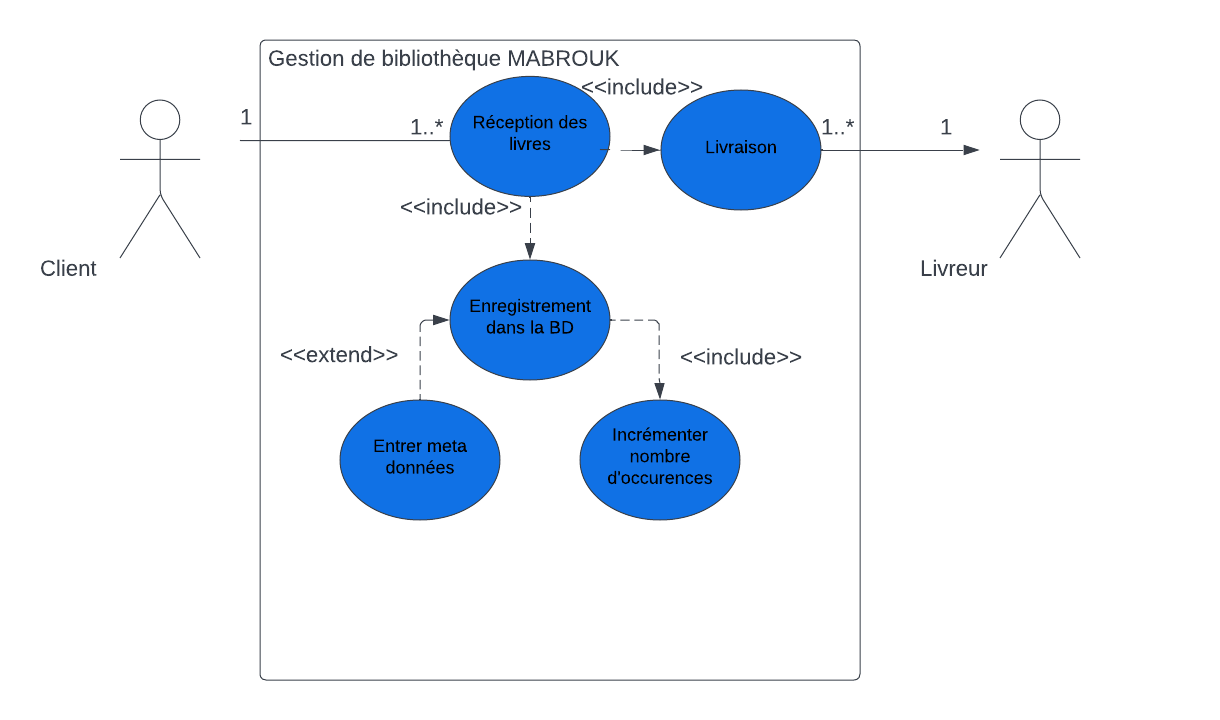
\includegraphics[scale=0.75]{capture1_S_1.png}
				%\caption{Légende de l'image}
			\end{figure}
			\item[b. ] L’emprunt et la restitution d’un ou plusieurs livres. On notera que le nombre
			maximum de livres pouvant être empruntés est de 5. Que ce soit pour l’emprunt ou
			la restitution, cela pourra être fait avec le bibliothécaire où une borne automatique.
			\newpage
			\begin{figure}[!hbtp]
				%\centering
				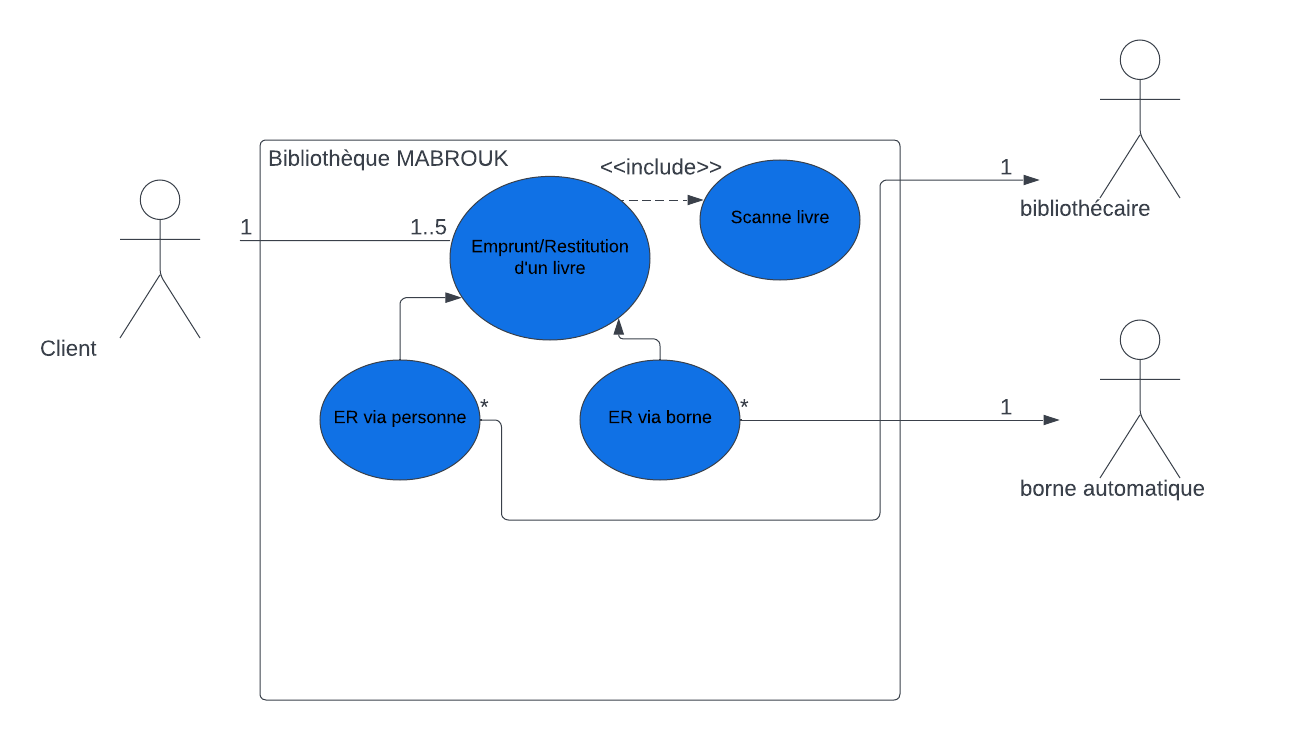
\includegraphics[scale=0.75]{capture2_S.png}
				%\caption{Légende de l'image}
			\end{figure}
		\end{itemize}
	\item[2. ] On souhaite modéliser le fonctionnement d’un restaurant dans les cas suivants :
	\begin{itemize}
		\item[a. ] À la prise de commande du client.\\preparation pour les cuisinier
		\item[b. ] Au paiement d’une table.\\paiement en especes,paiement par carte
	\end{itemize}
	\end{itemize}
\end{document}